%==============================================================================
%== template for LATEX poster =================================================
%==============================================================================
%
%--A0 beamer slide-------------------------------------------------------------
\documentclass[final]{beamer}
\usepackage[orientation=portrait,size=a0,
            scale=1.25         % font scale factor
           ]{beamerposter}
           
\geometry{
  hmargin=2.5cm, % little modification of margins
}

%
\usepackage[utf8]{inputenc}

\linespread{1.15}
%
%==The poster style============================================================
\usetheme{sharelatex}

%==Title, date and authors of the poster=======================================
\title
[CS234 Poster Session] % Conference
{ % Poster title
Replication Review for Coordinated Exploration in
Concurrent Reinforcement Learning
}

\author{ % Authors
Ed Fancher\inst{1}, 
}
\institute
[Stanford University] % General University
{
\inst{1} Department of Computer Science Stanford University, Stanford, California
}
\date{\today}



\begin{document}
\begin{frame}[t]
%==============================================================================
\begin{multicols}{3}
%==============================================================================
%==The poster content==========================================================
%==============================================================================

\section{Introduction}
These approaches may not always extend well to multiple agent settings. There are 2 single agent methods which have had some success: Upper Control Bound \cite{UCB2010} and PSRL (Bayesian) methods \cite{Strens2000} There have been recent attempts to extend these approaches to multi agent settings.

In this project, I attempt to replicate the findings in \cite{SeedSampling}. In this paper 3 approaches are compared: UCB based multiple agent approaches, Thompson Sampling and seed sampling. Seed sampling is based on the single agent PSRL approach.  In the UCB approach, as presented in the paper, the agents do not coordinate directly on exploration. Instead, they maintain a shared prior  and at the the beginning of an episode will generate an MDP model using an upper control bound approach.  Two agents, for which the shared prior is currently the same, will construct the same MDP and thus will have the same policy for the episode.

\begin{itemize}
\item Adaptivity

Adapt as data becomes available to make effective use of new
information.

\item Commitment

Maintain the intent to carry out probing action sequences
that span multiple periods.

\item Diversity

Divide-and-conquer learning opportunities among agents.

\end{itemize}

\subsection{Methods Compared}
\begin{itemize}
\item UCB
\item Thompson Sampling
\item Seed Sampling
\end{itemize}

\subsection{Scenarios}
\begin{itemize}
\item Bipolar chain

\vskip1ex
\begin{figure}
  \centering
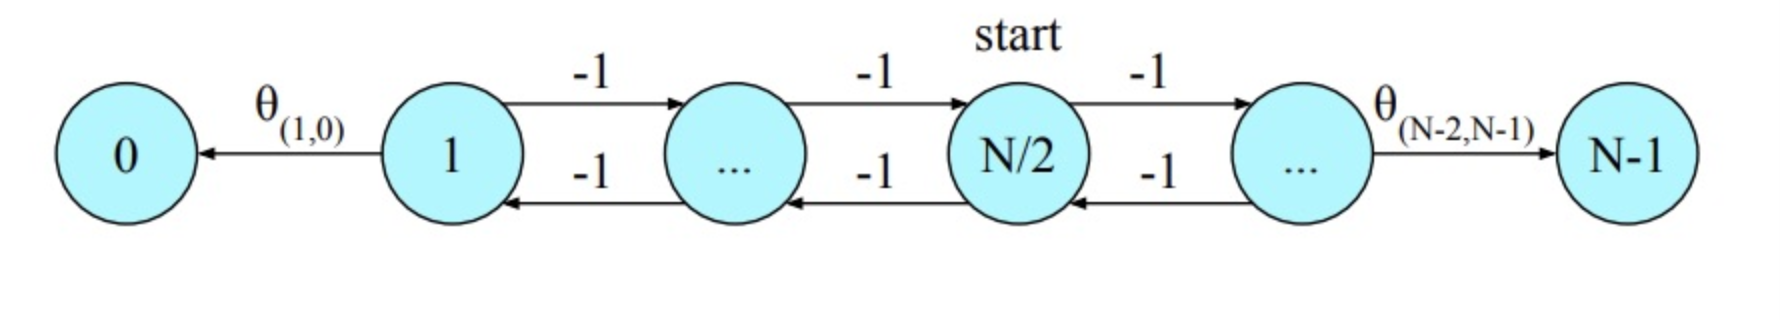
\includegraphics[scale=.75]{../project_update/bipolarchain.png}

  \caption{Graph of Bipolar Chain Example.}
 \label{fig:bipolarchain}
 
\end{figure}
\vskip2ex

\item Parallel chains

\vskip1ex
\begin{figure}
  \centering
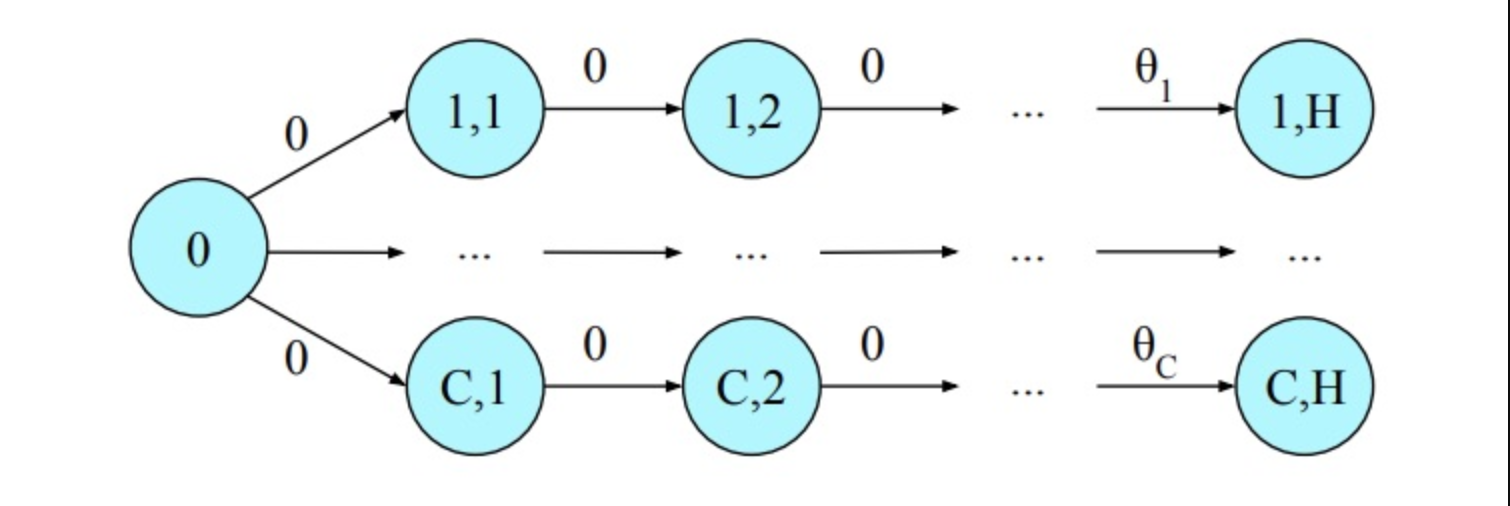
\includegraphics[scale=.75]{../project_update/parallelchains.png}

  \caption{Graph of Parallel Chains Example.}
 \label{fig:parallelchains}
\end{figure}
\vskip2ex

\item Maximum Reward Path

Erd\~os-R\'enyi graph

\end{itemize}
\section{Result and discussions}

\subsection{Bipolar Chain}
\begin{figure}[htbp!]
  \centering
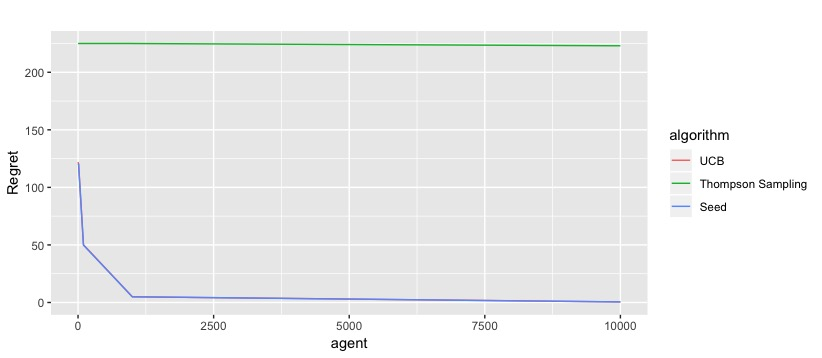
\includegraphics[scale=.75]{../project_update/results_pre.jpeg}

  \caption{Bipolar Chain Regret per Agent Count by Algorithm Type.}
 \label{fig:bipolarregretperagentbyalgo}
\end{figure}
As you can see in \ref{fig:bipolarregretperagentbyalgo} Both UCB (hidden under seed sampling) and seed sampling perform much better on Bipolar chain. Thompson sampling thrashes back and forth between a few states for the whole horizon.

\subsection{Parallel Chains}
\begin{figure}[htbp!]
  \centering
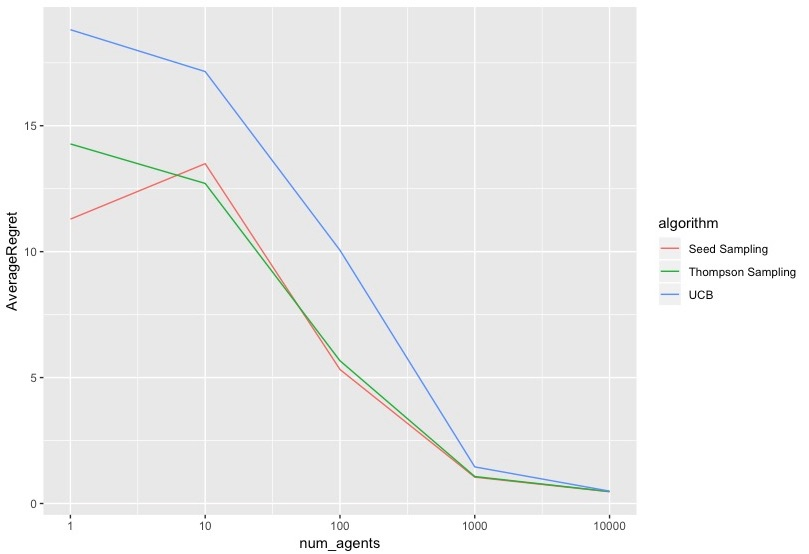
\includegraphics[scale=.75]{../project_update/pc_results_regret_by_algo.jpg}

  \caption{Parallel Chain Regret per Agent Count by Algorithm Type.}
 \label{fig:pc_results_regret_by_algo}
\end{figure}

\ref{fig:pc_results_regret_by_algo} shows that Thompson sampling and seed sampling outperform UCB for the parallel chains scenarior, only converging with a very large number of agents.

\begin{figure}[htbp!]
  \centering
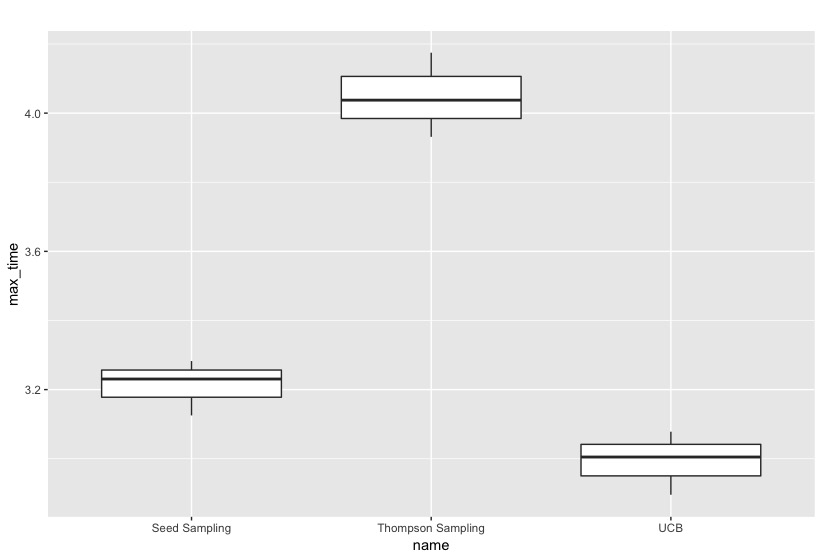
\includegraphics[scale=.75]{../project_update/pc_max_time_per_ag_by_algo.jpg}

  \caption{Parallel Chain Time (in minutes) per Run for 10000 Agents by Algorithm Type.}
 \label{fig:pc_max_time_per_ag_by_algo}
\end{figure}
The timing figure: \ref{fig:pc_max_time_per_ag_by_algo} shows that seed sampling is much faster than Thompson sampling despite having comparable performance on parallel chains.

\subsection{Maximum Reward Path}
\begin{figure}[htbp!]
  \centering
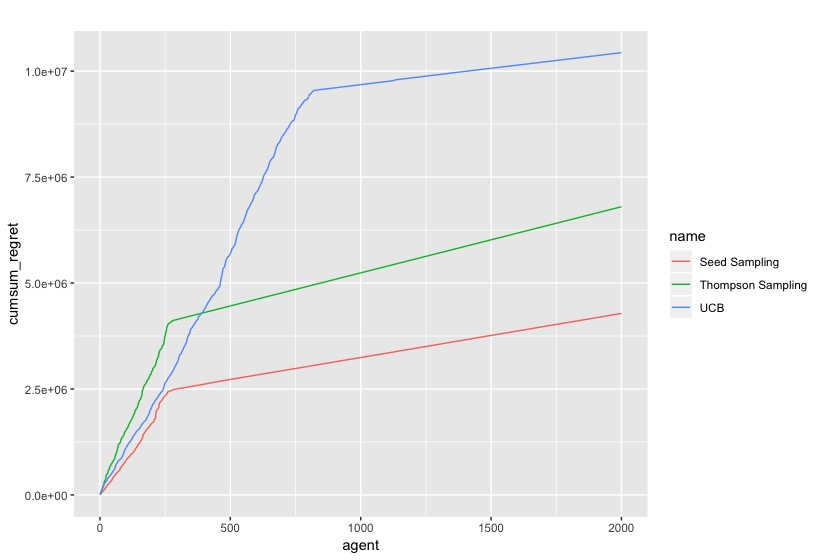
\includegraphics[scale=.75]{../project_update/mr_regret_per_ag_per_algo.jpg}
  \caption{Maximum Reward Path Regret per Agent Count by Algorithm Type.}
 \label{fig:mr_regret_per_ag_per_algo}
\end{figure}

Seed sampling performed really well in this scenario, having much lower average regret than both Thompson sampling and UCB.

\begin{figure}[htbp!]
  \centering
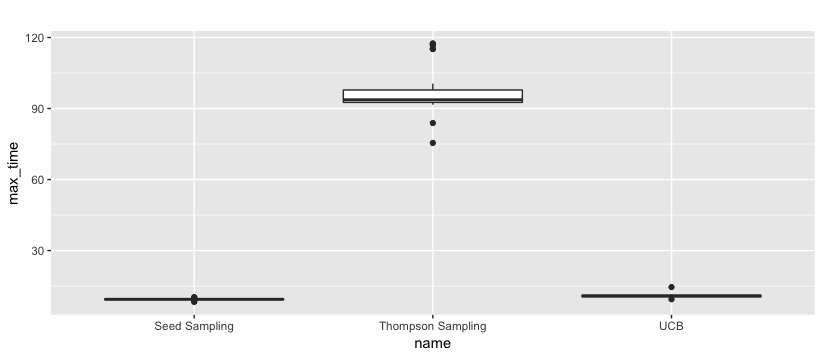
\includegraphics[scale=.75]{../project_update/mr_max_time_per_ag_by_algo.jpg}

  \caption{Maximum Reward Path Time (in minutes) per Run for 2000 Agents by Algorithm Type.}
 \label{fig:mr_max_time_per_ag_by_algo}
\end{figure}
As shown in Figure \ref{fig:mr_max_time_per_ag_by_algo}, seed sampling shows computation performance comparable to UCB, which makes sense since both solve MDPs at an episode start. This makes the time seed sampling and UCB take scale according to the number of episodes and agents, instead of the time steps for all agents.
\section{Conclusion}

I was able to replicate the findings in the paper. The results aren't exactly the same, but that isn't too surprising given that they aren't specific about the algorithms they compared against. What was really impressive was the gain in computational efficiency by reducing how often MDPs need to be solved. In all cases, seed sampling was much faster than thompson sampling, scaling as the number of episodes vs. the number of time steps. Yet, seed sampling retained much of the benefits of Thompson sampling in terms of providing exploration diversity.


\section{Future Work}
As mentioned above, the ideas here seem to be similar to adding noise to training images to improve generalization. It makes me think that it's likely this idea could be taken out of the Bayesian context and applied to algorithms like UCB1 or MSIE-EB, especially if the PAC guarantees of MSIE-EB could be retained. It seems likely that such a method would use something similar to how you would implement the ensembles mentioned in the \cite{SCALSS} paper.


%==============================================================================
%==End of content==============================================================
%==============================================================================

%--References------------------------------------------------------------------

\subsection{References}
\bibliography{project_update}
\bibliographystyle{icml2018}
\end{multicols}

%==============================================================================
\end{frame}
\end{document}
